%!TEX root=../hearts-revised.tex
\section{Hearts of $J$-slicings.}\label{hearts}
\begin{modifyepigraph}{.9}
\epigraph{I watched a snail crawl along the edge of a straight razor. That's my dream. That's my nightmare. Crawling, slithering, along the edge of a straight razor\dots\ and surviving.
}{Col. W\@. E\@. Kurtz}
\end{modifyepigraph}

Recall the equivalence relation $x\sim y$ if and only if there are integers $a,b \in \Z$ with $a\leq b$ such that $x + a \le y \le x + b$ on a $\Z$-toset $J$ from lemma \refbf{equivalence}.
\begin{lemma}\label{heartability}
The following are equivalent:
\begin{enumerate}[label=$\roman*$)]
\item the  $\Z$-toset $J$ consists of a single equivalence class with respect to the equivalence relation $\sim$; 
\item there exists an interval $I$ in $J$ such that the map $\varphi\colon (n,x)\mapsto x+n$ is an isomorphism of $\Z$-tosets $\Z\times_{\mathrm{lex}}I\xrightarrow{\sim} J$ (where the $\Z$-action on $I$ is the trivial one and the $\Z$-action on $\Z$ is the translation).
\end{enumerate}
\end{lemma}
\begin{proof}
That $(i)$ implies $(ii)$ is an immediate consequence of \refbf{lemma.representatives}. To prove the converse implication notice that since $\varphi$ is surjective every element in $J$ is equivalent to an element in $I$. So we are reduced to show that all elements in $I$ are equivalent each other. Let $x,y\in I$. We can assume $x\leq y$. Since $J$ is totally ordered we have either $y\leq x+1$ or $x+1\leq y$. In the latter case we have $x\leq x+1\leq y$ and so $x+1\in I$, since $I$ is an interval. But then $\varphi(1,x)=\varphi(0,x+1)$ against the hypothesis on $\varphi$. So we are left with $x\leq y\leq x+1$ which implies $x\sim y$.  
\end{proof}
\begin{definition}
Let $J$ be a $\Z$-toset. A \emph{heart} for $J$ is an interval $J^\heart\subseteq J$ such that $\varphi\colon (n,x)\mapsto x+n$ is an isomorphism of $\Z$-tosets $\Z\times_{\mathrm{lex}}J^\heart \xto{\sim} J$.
\end{definition}
\begin{remark}\label{hasaheart}
Of course, not every $\Z$-toset has a heart. It is easy to see that $J$ has an heart if and only if there is a morphism of $\Z$-tosets $\pi_\heart\colon J \to \Z$. An heart of $J$ is given by $\pi_\heart^{-1}(0)$ in this case.
\end{remark}
\begin{remark}
It is immediate from the definition that $J^\heart$ is a heart of $J$ if and only if $J^\heart+n$ is a heart of $J$, for every $n\in \Z$.
\end{remark}
\begin{example}
If $J=\Z$, with the standard $\Z$-toset structure, the hearts of $J$ are the singletons $\{n\}$ with $n\in \Z$. In particular $\{0\}$ is the standard heart of $\Z$, and all the other hearts are shifts of this. If $J=\mathbb{R}$, with the standard $\Z$-toset structure, then the hearts of $J$ are the intervals of the form $[x,x+1)$ and those of the form $(x,x+1]$, with $x\in \mathbb{R}$.
\end{example}

\begin{example}\label{I.has.a.heart}
Let $(J, \leq)$ be a totally ordered $\mathbb{Z}$-poset, and let $\sim$ be the equivalence relation from Lemma \refbf{equivalence}. For every $i\in J$ let $I_i$ be the equivalence class of $i$. This is an interval in $J$, see Example \refbf{class.is.interval}. Moreover, by Lemma \refbf{lemma.representatives}, $I_i$ has a heart precisely when $i$ is not a fixed point of the $\Z$-action.
\end{example}

\begin{lemma}\label{lemma.plus.one}
Let $I\colon \uno \to \O(J)$ be a heart of $J$. Then $I(1)=I(0)+1$, i.e., $U_1=U_0+1$ (equivalently, $L_1=L_0+1$).
\end{lemma}
\begin{proof}
Assume $U_1\nsubseteq U_0+1$. Then there exists an element $x$ in $U_1\cap(L_0+1)$. Since $I$ is a heart, there exists an element $y$ in $I$ and an integer $n$ such that $x=y+n$. If $n\geq 1$ we have $y+n\in U_0+n\subseteq U_0+1$ and so $x\in (U_0+1)\cap (L_0+1)$, which is impossible. If $n\leq 0$ we have $y+n\in L_1+n\subseteq L_1$ and so $x\in L_1\cap U_1$ which again is impossible. Therefore $U_1\subseteq U_0+1$. Now assume $U_0+1\nsubseteq U_1$. Then there exists an element $x\in (U_0+1)\cap L_1$. Let $y=x-1$. Then $y\in U_0\cap (L_1-1)\subseteq U_0\cap L_1=I$. Since $U_0+1\subseteq U_0$ we also have $x\in I$, and so $\varphi(-1,x)=\varphi(0,y)$, which is impossible. Therefore $U_1= U_0+1$.
\end{proof}
\begin{definition}
Let $J^\heart\subseteq J$ be a heart of $J$ and let $\tee\colon \O(J)\to  \ts(\C)$ be a $J$-slicing on a stable $\infty$-category $\C$. The subcategory $\C_{J^\heart}$ of $\C$ will be called a \emph{heart} of the $J$-slicing $\tee$ and will be denoted $\C^\heart$.
\end{definition}
\begin{notat}
We denote the canonical projection to the heart as $\mathcal{H}^\heart\colon \C\to \C^\heart$; see \adef\refbf{def.homology}.
\end{notat}
\begin{example}
We have seen in Example\refbf{ex.Z-is-t} that a  a $\Z$-slicing on a stable $\infty$-category $\C$ is the same thing as the datum of a $t$-structure $\tee=(\C_{<0},\C_{\geq 0})$ on $\C$. The standard heart $\C^\heart=\C_{\{0\}}$ is called the heart of the $t$-structure $\tee$. The projection to the heart is the functor $\mathcal{H}^0$; see Notation \refbf{Hi}.
\end{example}

From \refbf{cor:perPostnikov} we immediately get the following
\begin{proposition}\label{cor.oss.for.Heart.to.t}
Let $\tee=(\C_{<0},\C_{\geq 0})$ be a bounded $t$-structure on a stable $\infty$-category $\C$, and let $\C^\heart=\C_0$ be its standard heart. Then $\tee$ is completely determined by the functors $\mathcal{H}^j\colon \C \to \C^\heart[j]$ (and so by the functor $\mathcal{H}^0$ alone). More precisely, $\C_{\geq 0}$ is the full subcategory of $\C$ on the objects $Y$ such  that $\mathcal{H}^jY=0$ for any $j< 0$, while $\C_{< 0}$ is the full subcategory of $\C$ on those objects $Y$ for which $\mathcal{H}^jY=0$ for any $j\geq 0$.
\end{proposition}


\begin{remark}\label{evocative}
There is a rather evocative pictorial representation of the heart $\C_{[0,1)}$ of an $\mathbb{R}$-slicing, manifestly inspired by \cite{Brid}: if we depict $\C_{<0}$ and $\C_{\geq 0}$ as contiguous half-planes (refer to Figure \refbf{figure:slices})
then the action of the shift functor can be represented as an horizontal shift, and the closure properties of the two classes $\C_{<0}, \C_{\geq 0}$ under positive and negative shifts are a direct consequence of the shape of these areas. With these notations, an object $Z$ is in the heart $\C_{[0,1)}$ if it lies in a ``boundary region'', \ie if it lies in $\C_{\geq 0}$, but $Z[-1]$ lies in $\C_{<0}$.
\begin{center}
\begin{figure}[h]
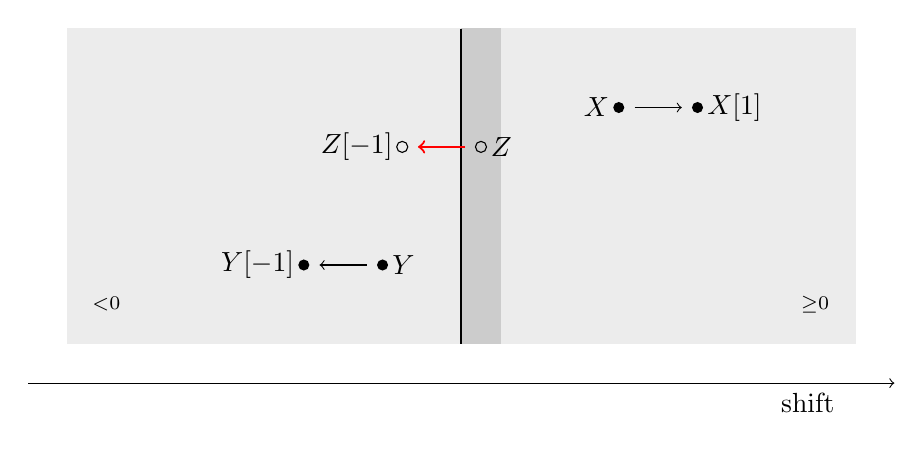
\begin{tikzpicture}
\filldraw[gray!15] (5,-2) -- (-5,-2) -- (-5,2) -- (5, 2) -- cycle;
\filldraw[gray!40] (.5, -2) -- (0,-2) -- (0,2) -- (.5,2) -- cycle;
\draw[thick] (0,-2) -- (0,2);
\fill (2,1) circle (2pt) node[left] (X) {$X$};
\fill (-1,-1) circle (2pt) node[right] (Y) {$Y$};
\node at (4.5,-1.5) {$\C_{\geq 0}$};
\node at (-4.5,-1.5) {$\C_{<0}$};
\draw[->] (2.2,1) -- (2.8,1);
\draw[->] (-1.2,-1) -- (-1.8,-1);
\fill[xshift=1cm] (2,1) circle (2pt) node[right] (X) {$X[1]$};
\fill[xshift=-1cm] (-1,-1) circle (2pt) node[left] (Y) {$Y[-1]$};
\draw (.25,0.5) circle (2pt) node[right] {$Z$};
\draw (-.75,0.5) circle (2pt) node[left] {$Z[-1]$};
\draw[thick, ->, red] (.05,0.5) to (-.55,0.5);
\draw[->, xshift=-.5cm, yshift=-.5cm] (-5,-2) -- (6,-2) node[below, pos=.9] {\text{shift}};
\end{tikzpicture}
\caption{Heart of an $\mathbb{R}$-slicing}
\label{figure:slices}
\end{figure}
\end{center}
\end{remark}


Let now $J^\heart\subseteq J$ be a heart, and let $\C^\heart=\C_I$ be the corresponding subcategory of $C$, relative to a given $J$-slicing $\tee$. Writing $I$ as $I\colon \uno \to \O(J)$, for any $n\in \Z$ and any $k\geq 0$ we can consider the interval decomposition $I_{\ordered{k}}\colon \ordered{k}\to \O(J)$ defined by setting $I_{\ordered{k}}(j)=I(0)+j+n$ for $0\leq j\leq k$. By Lemma \refbf{lemma.plus.one}, this corresponds to the collection of $n$ contiguous intervals $I+n,I+n+1,\dots,I+n+k-1\subseteq J$. The corresponding subcategories of $\C$ will be $\C^\heart[n]$, $\C^\heart[n+1]$,\dots,$\C^\heart[n+k-1]$.



 The existence and uniqueness of $I_{\ordered{k}}$-weaved factorizations then specializes to the following statement
\begin{proposition}\label{prop.first-tower}
Let $f\colon X\to Y$ be a morphism in $\C$. Then for any integer $n$ and any positive integer $k$ there exists a unique factorization
\[
X \xto{f_{n+k}} Z_{n+k-1} \xto{f_{n+k-1}}Z_{n+k-2}\to\dots\to Z_{n+1} \xto{f_{n}} Z_{n} \xto{f_{n-1}} Y,
\]
of $f$ such that
$\cofib(f_j)\in \C^\heart[j]$ for any $j=n,\dots,n+k-1$,  $\cofib(f_{n-1})\in \C_{L_0}[n]$  and $\cofib(f_{n+k})\in \C_{U_k}[n]=\C_{U_0}[k+n]$.
\end{proposition}
The content of \aprop\refbf{prop.first-tower} becomes more interesting when $\C$ is \emph{bounded} with respect to the $J$-slicing $\tee$ (see \adef\refbf{def.bounded}), as in this case $\cofib(f)$ lies in $\C_{U_0}[n]$ for $n\ll 0$ and in $\C_{L_0}[n]$ for $n\gg0$ . Namely, if $\C$ is $J$-bounded, then $\cofib(f)$ lies in $\C_{\geq i}$ for some $i\in J$. Since $J^\heart$ is a heart, there exists an element $x\in I$ and an integer $n_0$ such that $i=x+n_0$, so that $\cofib(f)\in \C_{\geq x}[n_0]$. As $x\in I$ we have $x\in U_0$ and so $[x,+\infty)\subseteq U_0$ therefore $\cofib(f)\in \C_{U_0}[n_0]$ and so $\cofib(f)\in \C_{U_0}[n]$ for any $n\leq n_0$. Dually one proves the statement for $n\gg0$. 
 As an immediate consequence, by Remark \refbf{rem.trivial-factorizations} we see that in the $J$-bounded case
if $f\colon X\to Y$ is any morphism in $\C$, then  
 the morphisms $0 \to \cofib(f)_{n+k-1}$ and $\cofib(f)_{n} \to \cofib(f)$ in $\rook\Big(\varnobkt{0}{\cofib(f)},I_{\ordered{k}}\Big)$ are isomorphisms for $n\ll 0$ and $k \gg 0$. Since $\rook\Big(\varnobkt{0}{\cofib(f)},I_{\ordered{k}}\Big)$ is the $I_{\ordered{k}}$-weaved factorization of $0\to \cofib(f)$ by Corollary \refbf{cor:perPostnikov}, and since isomorphisms are preserved by pullouts we see that both $X \xto{f_{n+k}} Z_{n+k-1} $ and $Z_{n} \xto{f_{n-1}} Y$ are isomorphisms.
 
 %One notices, as it is obvious, that the class of isomorphisms in $\C$ is closed under transfinite composition 
 \par
 This leads to the following
\begin{proposition}\label{prop.Z.Postnikov}
Let $\C$ be a stable $\infty$-category which is bounded with respect to a given $J$-slicing $\tee$. Let $J^\heart\subseteq J$ be a heart for $J$ and let $\C^\heart$ be the corresponding heart in $\C$.
Then for any morphism $f\colon X\to Y$  in $\C$ there exists an integer $n_0$ and a positive integer $k_0$ such that for any integer $n\leq n_0$ and any positive integer $k$ with $k\geq n_0-n+k_0$ there exists a unique factorization of $f$ 
\[
X \xto{\sim} Z_{n+k-1} \xto{f_{n+k-1}}Z_{n+k-2}\to\dots\to Z_{n+1} \xto{f_{n}} Z_{n} \xto{\sim} Y
\]
such that
$\cofib(f_j)\in \C^\heart[j]$ for any $j=n,\dots,n+k-1$.
\end{proposition}
\begin{remark}\label{oss.Z.Postnikov}
By uniqueness in \aprop\refbf{prop.Z.Postnikov}, one has a well defined $\Z $-factorization
\[
X=\lim(Z_j) \to\cdots \to Z_{j+1} \xto{f_{j}} Z_{j} \xto{f_{j-1}}Z_{j-1}\to \cdots\to \mathrm{colim}(Z_j)=Y
\]
with $j$ ranging over the integers, $\cofib(f_j)\in \C^\heart[j]$ for any $j\in \Z $ and with $f_m$ being an isomorphism for $|j|\gg 0$. We will refer to this factorization as the $\C^\heart$-weaved factorization of $f$. Notice how the boundedness of $\C$ has played an essential role: when $\C$ is not bounded, one still has towers for interval decomposition $I_{\ordered{k}}\colon j\mapsto I(0)+j+n$ for arbitrary $k$ and $n$, but in general they do not stabilize.
\end{remark}
\begin{remark}\label{oss.for.Heart.to.t}
Let $J^\heart\subseteq J$ be a heart, and let $(L,U)$ be the slicing $J^\heart(0)$ of $J$ and $\tee=(\C_U,\C_L)$ be the corresponding $t$-structure on $\C$. By Lemma \refbf{lemma.plus.one} the standard heart of $\tee$ is precisely $\C^\heart$. Moreover,
by Corollaries \refbf{cor:perPostnikov} and \refbf{perPostnikov2}, the $\C^\heart$-weaved factorization 
\[
0=\lim(Y_j) \to\cdots \to Y_{j+1} \xto{f_{j}} Y_{j} \xto{f_{j-1}}Y_{j-1}\to \cdots\to \mathrm{colim}(Y_j)=Y
\]
of an initial morphism $0\to Y$ is such that $\cofib(f_j)=\mathcal{H}^jY$ for any $j\in \Z$. Therefore we see that the $t$-structure $(\C_L,\C_U)$ can be completely read from $\C^\heart$-weaved factorizations: an object $Y$ is in $\C_{U}$ if and only if the $\C^\heart$-weaved factorization of $0\to Y$
satisfies $\cofib(f_j)=0$ for any $j< 0$, while $Y$ is in $\C_{L}$ if and only if  $\cofib(f_j)=0$ for any $j\geq 0$. We are going to use this fact later to characterize hearts of $t$-structures among full subcategories of $\C$.
\end{remark}

\begin{remark}\label{bounded.is.bounded}
The content of Remark \refbf{oss.for.Heart.to.t} can be elegantly expressed in terms of the functoriality of slicings (Remark \refbf{rem.slicing-functor}). Namely, by Remark \refbf{hasaheart}, to give a heart $J^\heart$ of $J$ is equivalent to giving  a $\Z$-equivariant morphism of $\pi_\heart\colon \Z$-tosets $J\to\Z$, and by functoriality this induces a map
\[
\pi_\heart\colon \slicings(J,\C)\to \ts(\C).
\]   
The heart $\C^\heart$ of a $J$-slicing $\tee$ on $\C$ is then the standard heart of the corresponding $t$-structure $\pi_\heart(\tee)$. Moreover, one easily sees that $\tee$ is a bounded $J$-slicing if and only if $\pi_\heart(\tee)$ is a bounded $t$-structure. Indeed, since $\pi_\heart$ is a morphism of tosets, for any $i_1\leq i_2$ in $J$ we have $[i_1,i_2]\subseteq \pi_\heart^{-1}[\pi_\heart(i_1),\pi_\heart(i_2)]$. Vice versa, since  $\pi_\heart$ is $\Z$-equivariant, for every $j\in J$ we have $\pi_\heart(j+n)=\pi_\heart(j)+n$ and so for every $n_1\leq n_2$ in $\Z$ there exist $j_1\leq j_2$ in $J$ such that $\pi_\heart(j_1)< n_1$ and $\pi_\heart(j_2)> n_2$. Let $j\in J$ be such $n_1\leq \pi_\heart(j)\leq n_2$. If $j>j_2$ then we would have $\pi_\heart(j)\geq \pi_\heart(j_2)>n_2$, and so $j\leq j_2$. Similarly $j\geq j_1$ and so $\pi_{\heart}^{-1} [n_1,n_2]\subseteq [j_1,j_2]$.
\end{remark}


\subsection{Abelianity of the heart.}
In the following section we present a proof of the fact that a heart $\C^\heart$ of a $J$-slicing on a stable $\infty$-category $\C$
is an abelian $\infty$-category. 

In other words, $\C^\heart$ is homotopy equivalent to its homotopy category $h\C^\heart$, which is an abelian category; this is the higher-categorical counterpart of a classical result, first proved in \cite[\athm\textbf{1.3.6}]{BBDPervers}, 
which 
only relies on properties stated in terms of normal torsion theories in a stable $\infty$-category. 

We begin with the following
\begin{definition}[Additive $\infty$-category]\label{df:additive}
An \emph{additive $\infty$-category}  is an additive
category regarded as an $\infty$-category.
\end{definition}
\begin{remark}
Equivalently, an additive $\infty$-category is a quasicategory $\cate{A}$
such that
\begin{enumerate}[label=$\roman*$)]
\item the hom space $\cate{A}(X,Y)$ is a homotopically discrete infinite loop space for any $X, Y$, \ie, there exists an infinite sequence of $\infty$-groupoids $\Xi_0, \Xi_1,\Xi_2,\dots$, with $\Xi_0\cong \C(X,Y)$ and homotopy equivalences $\Xi_i\cong \Omega \Xi_{i+1}$ for any $i\geq 0$, such that $\pi_n \Xi_0=0$ for any $n\geq 1$;
\item $\cate{A}$ has a zero object, and (homotopy) biproducts.
\end{enumerate}
\end{remark}
\begin{remark}\label{orthogonality-of-a}
If $\cA$ is a full additive $\infty$-subcategory of a stable $\infty$-category $\C$, then $\cA[n_1]\orth\cA[n_2]$ for any $n_1>n_2$. Namely, for an additive $\cA$, let $X\in \cA[n_1]$ and $Y\in\cA[n_2]$. Then $X=Z_1[n_1]$ and $Y=Z_2[n_2]$ for suitable $Z_1,Z_2\in \cA$ and so 
\begin{align*}
\C(X,Y)&=\C(Z_1[n_1],Z_2[n_2])\cong  \C(Z_1,Z_2[n_2-n_1])\\
&\cong \Omega^{n_1-n_2}\C(Z_1,Z_2)=\Omega^{n_1-n_2}\cA(Z_1,Z_2),
\end{align*}
where in the last equality we used the fact that $\cA$ is full. Since $n_1-n_2>0$, the space $\Omega^{n_1-n_2}\cA(Z_1,Z_2)$ is contractible by definition of additive $\infty$-category.
\end{remark}
\begin{remark}
In the triangulated setting one does not have the compatibility between the looping operation on objects and on spaces of morphisms $\Omega\C(X,Y)=\C(X,\Omega Y)$ and so the othogonality condition $\cA[n_1]\orth\cA[n_2]$ for $n_1>n_2$, when needed, has to be imposed by hands. This is nothing but the usual vanishing of negative Ext's one frequently meets as a property of `good' additive subcategories of a triangulated category.  
\end{remark}

\begin{definition}[Abelian $\infty$-category]\label{df:abelinfty}
An \emph{abelian $\infty$-category}  is an abelian
category regarded as an $\infty$-category.
\end{definition}
\begin{remark}
Equivalently, an abelian $\infty$-category is an additive $\infty$-category $\cate{A}$
such that
\begin{enumerate}[label=$\roman*$)]
\item $\cate{A}$ has (homotopy) kernels and cokernels;
\item for any morphism $f$ in $\cate{A}$, the natural morphism from the \emph{coimage} of $f$ to the \emph{image} (see \adef\refbf{imcoim}) of $f$ is an equivalence.
\end{enumerate}
\end{remark}
%\begin{remark}
%Axiom (i) is the homotopically-correct version of $\cate{A}(X,Y)$ being an abelian group. For instance, if the abelian group is $\Z $, then the corresponding homotopy discrete space is the Eilenberg-Mac Lane spectrum $\Z ,K(\Z ,1), K(\Z ,2),\dots$. The homotopy category of such an $\cate{A}$ is an abelian category in the classical sense (note that $\cate{A}(X,Y)$ being homotopically discrete is necessary in order that kernels and cokernels in $\cate{A}$ induce kernels and cokernels in $h\cate{A}$). Moreover, since the hom spaces $\cate{A}(X,Y)$ are homotopically discrete, the natural morphism $\cate{A}\to h\cate{A}$ is actually an equivalence.
%\end{remark}

The rest of the section is devoted to the proof of the following result:
\begin{theorem}\label{heart.is.abelian}
Let $\C^\heart$ be a heart of a $J$-slicing $\tee$ on a stable $\infty$-category $\C$. Then $\C^\heart$ is an abelian $\infty$-category.\end{theorem}
\begin{remark}
If $J=\Z$, so that $\tee$ is the datum of a $t$-structure on $\C$, and $\C^\heart=\C_{\{0\}}$ is the standard heart of $\C$, the the  homotopy category $h\C^\heart$ is the abelian category arising as the standard heart of the $t$-structure $h(\tee)$ on the triangulated category $h\C$.
\end{remark}
In what follows, let $I\colon \uno \to \O(J)$ be an interval such that $\C^\heart=\C_I$. The two factorization systems associated with $I$ will be denoted by $(\E_0,\M_0)$ and $(\E_1,\M_1)$, respectively. By Lemma \refbf{lemma.plus.one} we have $\M_1=\M_0[1]$ and $\E_1=\E_0[1]$.
\begin{lemma}
For any $X$ and $Y$ in $\C^\heart$, the hom space $\C^\heart(X,Y)$ is a homotopically discrete infinite loop space.
\end{lemma}
\begin{proof}
Since $\C^\heart$ is a full subcategory of $\C$, we have $\C^\heart(X,Y)=\C(X,Y)$, which is an infinite loop space since $\C$ is a stable $\infty$-category. 

So we are left to prove that $\pi_n\C(X,Y)=0$ for $n\geq 1$. Since $\pi_n\C(X,Y)=\pi_{n-1}\Omega\C(X,Y)=\pi_{n-1}\C(X,Y[-1])$, this is equivalent to showing that 
$\C(X,Y[-1])$ is contractible. Since $X$ and $Y$ are objects in $\C^\heart$, we have $X\in \C_{U_0}$ and $Y[-1]\in \C_{L_1[-1]}=\C_{L_1-1}=\C_{L_0}$. But $\C_{L_0}$ is right object-orthogonal to $\C_{U_0}$, therefore $\C(X,Y[-1])$ is contractible.
\end{proof}

The subcategory $\C^\heart$ inherits the $0$ object and biproducts (in fact, all finite limits) from $\C$, so in order to prove it is is abelian we are left to prove that it has kernels and cokernels, and that the canonical morphism from the coimage to the image is an equivalence.
\begin{lemma}\label{lemma.qua.e.la}
Let $f\colon X\to Y$ be a morphism in $\C^\heart$. Then $\mathrm{fib}(f)$ is in $\C_{L_1}$ and $\cofib(f)$ is in $\C_{U_0}$.
\end{lemma}
\begin{proof}
Since both $X\to 0$ and $Y\to 0$ are in $\M_1$, by the 3-for-2 property also $f$ is in $\M_1$. Since $\M_1$ is closed for pullbacks, $\mathrm{fib}(f)\to 0$ is in $\M_1$ and so $\mathrm{fib}(f)$ is in $\C_{L_1}$. The proof for $\cofib(f)$ is completely dual.
\end{proof}
\begin{definition}
Denote by
\[
\xymatrix{
0\ar[r]^-{\E_0}&\ker(f)\ar[r]^{\M_0}&\fib(f)
}
\]
the $(\E_0,\M_0)$-factorization of the morphism $0\to \fib(f)$
and by
\[
\xymatrix{
\cofib(f)\ar[r]^{\E_1}&\coker(f)\ar[r]^-{\M_1} &0
}
\]
the $(\E_1,\M_1)$-factorization of the morphism $\cofib(f)\to 0$. We call $\ker(f)$ and $\coker(f)$ respectively the \emph{kernel} and the \emph{cokernel} of $f$ in $\C^\heart$.
\end{definition}
\begin{remark}\label{oss.miracle}
Since $\cofib(f)[-1]\cong \fib{f}$ and $(\M_1,\E_1)[-1]=(\M_0,\E_0)$, one can equivalently define $\coker(f)$ by declaring the $(\E_0,\M_0)$-factorization of $\fib(f)\to 0$ to be $\fib(f)\xto{\E_0}\coker(f)[-1]\xto{\M_0} 0$. Similarly, one can define $\ker(f)$ by declaring the $(\E_1,\M_1)$-factorization of $0\to \cofib(f)$ to be $0\xto{\E_1}\ker(f)[1]\xto{\M_1} \cofib(f)$.
By normality of the factorization system we therefore have the homotopy commutative diagram 
\[
\begin{kodi}
\obj{
	0  &|(ker)| \ker(f) &[1cm] |(fib)| \fib(f)\\
	&|(0')| 0 &|(coker)| \coker(f)[-1] & |(0'')| 0 \\
};
\mor 0 {\E_0}:-> ker \M_0:-> fib \E_0:-> coker \M_0:-> 0'';
\mor ker \E_0:-> 0' \M_0:-> coker \M_0:-> 0'';
\end{kodi}
\]
whose square sub-diagram is a homotopy pullout.
\end{remark}
\begin{lemma}
Both $\ker(f)$ and $\coker(f)$ are in $\C^\heart$.
\end{lemma}
\begin{proof}
By construction $\ker(f)$ is in $\C_{U_0}$, so we only need to show that $\ker(f)$ is in $\C_{L_1}$. By definition of $\ker(f)$, we have that $\ker(f)\to \fib(f)$ is in $\M_0$. Since $\M_0[-1]\subseteq \M_0$, we have that also $\ker(f)[-1]\to \fib(f)[-1]$ is in $\M_0$.
By Lemma \refbf{lemma.qua.e.la}, $\fib(f)[-1]\to 0$ is in $\M_1[-1]=\M_0$ and so we find that also $\ker(f)[-1]\to 0$ is in $\M_0$. 
The proof for $\coker(f)$ is perfectly dual.
\end{proof}
By definition of $\ker(f)$ and $\coker(f)$, the defining diagram of $\fib(f)$ and $\cofib(f)$ can be enlarged as
\[
\begin{kodi}
\obj{
0 & |(ker)| \ker(f) & |(fib)| \fib(f) & X & |(01)| 0 \\
& &|(02)| 0 & Y & |(cofib)| \cofib(f) & |(coker)| \coker(f) & |(03)| 0\\	
};
\mor 0 -> ker -> fib -> X -> 01 -> cofib -> coker -> 03;
\mor fib -> 02 -> Y -> cofib;
\mor X f:-> Y;
\mor ker k_f:{bend left=40},-> X; \mor Y c_f:swap,{bend right=40},-> coker;
\end{kodi}
\]
where $k_f$ and $c_f$ are morphisms in $\C^\heart$.
\begin{definition}\label{imcoim}
Let $f\colon X\to Y$ be a morphism in $\C^\heart$. The \emph{image} $\im(f)$ and the \emph{coimage} $\coim(f)$ of $f$ are defined as $\im(f)=\ker(c_f)$ and  $\coim(f)=\coker(k_f)$. 
\end{definition}
The following lemma shows that $\ker(f)$ does indeed have the defining property of a kernel:
\begin{lemma}\label{is.a.kernel}
The homotopy commutative diagram
\[
\xymatrix{
\ker(f)\ar[r]^{k_f}\ar[d]&X\ar[d]^{f}\\
0\ar[r]&Y}
\]
is a pullback diagram in $\C^\heart$.
\end{lemma}
\begin{proof}
A homotopy commutative diagram 
\[
\xymatrix{
K\ar[r]\ar[d]&X\ar[d]^{f}\\
0\ar[r]&Y}
\]
between objects in the heart is in particular a homotopy commutative diagram in $\C$ so it is equivalent to the datum of a morphism $k'\colon K\to \fib(f)$ in $\C$, with $K$ an object in $\C^\heart$. By the orthogonality of $(\E_0,\M_0)$, this is equivalent to a morphism $\tilde{k}\colon K\to\ker(f)$:
\[\xymatrix{
0\ar[r]\ar[d]_{\E_0}&\ker(f)\ar[d]^{\M_0}\\
K\ar[ru]^{\tilde{k}}\ar[r]_{k'}&\fib(f)
}. \qedhere 
\]
\end{proof}
There is, obviously, a dual result showing that $\coker(f)$ is indeed a cokernel.
\begin{lemma}
The homotopy commutative diagram
\[\xymatrix{
X\ar[r]\ar[d]_{f}&0\ar[d]\\
Y\ar[r]^-{c_f}&\coker(f)
}\]
is a pushout diagram in $\C^\heart$.
\end{lemma}

\begin{proposition}\label{pullout.is.pullout}
A homotopy commutative diagram
\[
\xymatrix{
X\ar[r]^{f}\ar[d]&Y\ar[d]_{g}\\
\zero\ar[r]&Z
}
\]
with vertices in $\C^\heart$ is a pullout diagram in $\C^\heart$ if and only if it is a pullout diagram in $\C$. 
\end{proposition}
\begin{proof}
Since $\C^\heart$ is a full subcategory of $\C$ it is clear that if the given diagram is a pullout in $\C$ then it is automatically also a pullout in $\C^\heart$. Conversely, assume the given diagram is a pullout in $\C^\heart$. This means that $X=\ker(g)$ and $Z=\coker(f)$. By definition of $\ker$ and $\coker$ this implies that we have the following homotopy commutative diagram in $\C$ where each square is a pullout (in $\C$):
\[
\begin{kodi}%[training wheels]
\obj{
   |(01)|\zero &[1cm]  X &[1cm]  \fib(g)  &[1cm] Y \\
&  |(02)|\zero &  W & \cofib(f)     \\
&& |(03)|\zero &  Z                 \\
%&&&|(04)|\zero.                     \\
};
\mor 01 \E_0:-> X \E_0:-> 02 -> W \E_0:-> 03 -> Z;% \M_1:-> 04;
\mor X \M_0:-> {fib g} \E_0:-> W -> {cofib f} \E_1:-> Z;
\mor {fib g} -> Y -> {cofib f};
\mor X f:dashed,{bend left},-> Y g:dashed,{bend left=50},-> Z;
\end{kodi}
\]
Here $X\to \zero$ is in $\E_0$ by definition of $\ker(g)$ and by the Sator lemma, and so also $\fib(g)\to W$ is in $\E_0$ since $\E_0$ is closed under pushouts.
The morphism $\cofib(f)\to Z$ is in $\E_1$ by definition of $\coker(f)$. From the pullout diagram in $\C$
\[
\xymatrix{
\cofib(f)\ar[r]\ar[d] & \zero\ar[d]\\
Z\ar[r] & W[1]
}
\]
 and the fact $\E_1$ is closed under pushouts that follows that $\zero\to W[1]$ is in $\E_1$. Therefore $\zero\to W$ is in $\E_1[-1]=\E_0$ and so $W\to \zero$ is in $\E_0$. This shows that $\fib(g)\to \zero$ is in $\E_0$ and so $X\to \fib(g)$ is an isomorphism. Therefore the given diagram is a pullback in $\C$ and so a pullout in $\C$. 
\end{proof}




\begin{lemma}\label{lemma.titanic}
For $f\colon X\to Y$ a morphism in $\C$, there is a homotopy commutative diagram where all squares are homotopy pullouts:
\[
\begin{kodi}
\obj{
|(ker)| \ker(f) &[1cm] |(fib)| \fib(f) &[1cm] X &[1cm] 0 &[1cm]\\
|(01)| 0 &|(coker-1)| \coker(f)[-1] & |(Z)| Z_f &|(ker1)| \ker(f)[1] &|(02)| 0 \\
& |(03)| 0 & Y & |(cofib)| \cofib(f) & |(coker)| \coker(f) \\
};
\mor ker -> fib -> X -> 0 {{\E_1}}:-> ker1 -> 02 {{\M_1}}:-> coker;
\mor ker {\E_0}:-> 01 -> coker-1 -> Z -> ker1 {{\M_1}}:-> cofib -> coker;
\mor fib {\E_0}:-> coker-1 {\M_0}:-> 03 -> Y -> cofib;
\mor[swap] X {\E_0}:-> Z {{\M_1}}:-> Y;
\mor X f:{near start},dashed,{bend left},-> Y; 
\mor ker k_f:{bend left},-> X; 
\mor[swap] Y c_F:{bend right},-> coker;
\end{kodi}\]
uniquely determining an object $Z_f\in \C^\heart$.
\end{lemma}
\begin{proof}
Define $Z_f$ as the homotopy pullout
\[
\xymatrix{
\fib(f)\ar[r]\ar[d]_{\E_0} \pp & X\ar[d]^{\E_0}\\
\coker(f)[-1]\ar[r]& Z_f}
\]
Here the vertical arrow on the right is in $\E_0$ since the vertical arrow on the left is in $\E_0$ by definition of $\coker(f)$ (see Remark \refbf{oss.miracle}) and $\E_0$ is preserved by pushouts. Next, paste on the left of this diagram the pullout given by Remark \refbf{oss.miracle} and build the rest of the 
diagram by taking pullbacks or pushouts, recalling that $(\E_0,\M_0)[1]=(\E_1,\M_1)$. Use again Remark \refbf{oss.miracle} and the fact that $\M_1$ is closed under pullbacks to see that $Z_f\to Y$ is in $\M_1$. 
Finally, we have 
\[
0\xto{\E_0} X\xto{\E_0} Z_f\xto{\M_1} Y\xto{\M_1} 0,
\]
and so $Z_f$ is in $\C^\heart$.
\end{proof}
\begin{proposition}\label{im.iso.coim}
There is an isomorphism $\im (f)\cong\coim (f)$.\end{proposition}
\begin{proof}
By definition, $\im(f)$ and $\coim(f)$ are defined by the factorizations
\[
\xymatrix{
0\ar[r]^-{\E_0}&\im(f)\ar[r]^{\M_0}&\fib(c_f)
}
\]
and
\[
\xymatrix{
\cofib(k_f)\ar[r]^{\E_1}&\coim(f)\ar[r]^-{\M_1} &0
}
\]
The diagram in Lemma \refbf{lemma.titanic} shows that we have $\fib(c_f)=Z_f=\cofib(k_f)$. Therefore, 
what we need to exhibit are the $(\E_0,\M_0)$ factorizations of $0\to Z_f$ and the $(\E_1,\M_1)$ factorization of $Z_f\to 0$. Since $Z_f$ is an object in $\C^\heart$, these are
\[
0\xrightarrow{\E_0}Z_f\xrightarrow{\mathrm{id}_{Z_f}}Z_f
\]
and 
\[
Z_f\xrightarrow{\mathrm{id}_{Z_f}}Z_f\xrightarrow{\M_1}0,
\]
respectively, thus giving $\im(f)\cong Z_f\cong \coim(f)$.
\end{proof}

\subsection{Abelian subcategories as hearts.}
By the results in the previous section and by Corollary \refbf{cor.oss.for.Heart.to.t} we see that hearts of bounded $t$-structures are very peculiar subcategories of a stable $\infty$-category $\C$: they are abelian and every morphism in $\C$ admits a unique $\C^\heart$-weaved factorization. As we are going to show, these two properties precisely characterize hearts among full subcategories of $\C$.
\begin{definition}
Let $f\colon X\to Y$ be a morphism in $\C$, and let $\cA$ be an additive $\infty$-subcategory of $\C$. An $\cA$-weaved factorization of $f$ is a factorization
\[
X=\lim(Z_j) \to\cdots \to Z_{j+1} \xto{f_{j}} Z_{j} \xto{f_{j-1}}Z_{j-1}\to \cdots\to \mathrm{colim}(Z_j)=Y
\]
with $j$ ranging over the integers, $\cofib(f_j)\in \cA[j]$ for any $j\in \Z $ and with $f_m$ being an isomorphism for $|j|\gg 0$.
\end{definition}

\begin{proposition}
Let $\cA$ be an additive full $\infty$-subcategory of a stable $\infty$-category $\C$ such that any morphism $f\colon X\to Y$  in $\C$ has an $\cA$-weaved factorization. Then the collection of subcategories $\{\cA[n]\}_{n\in \Z}$ is a Bridgeland $\Z$-slicing of $\C$.
\end{proposition}
\begin{proof} Looking at \adef\refbf{def.bridgeland-slicing}, the only thing we need to prove is that $\cA[n_1]\orth\cA[n_2]$ for $n_1>n_2$. This is Remark \refbf{orthogonality-of-a}.
\end{proof}


From Proposition \refbf{b-is-discrete} and Remark \refbf{rem:b-is-discrete} we then immediately have the following converse of Corollary \refbf{cor.oss.for.Heart.to.t}, corresponding to \cite[Lemma 3.2]{Brid}.
\begin{proposition}\label{to.be.repeated.verbatim}
Let $\cA$ be a full additive $\infty$-subcategory of a stable $\infty$-category $\C$, such that  any morphism in $\C$ has a $\cA$-weaved factorization, and let
$\mathcal{H}^n_B\colon \C\to \cA[n]$ be the functors given by taking the cofibers of the $n$-th morphism in the $\cA$-weaved factorization of the initial morphisms. 
 Let
$\C_{\cA,\geq 0}$ be the full subcategory of $\C$ on those objects $X$ such that $\mathcal{H}^j_B(X)=0$ for any $j< 0$, and let $\C_{\cA,< 0}$ be the full subcategory of $\C$ on those objects $X$ such that $\mathcal{H}^j_B(X)=0$ for any $j\geq 0$. Then $\mathfrak{t}_{\cA}=(\C_{\cA,\geq 0}, \C_{\cA,<0})$ is a $t$-structure on $\C$, the stable $\infty$-category $\C$ is bounded with respect to $\mathfrak{t}_{\cA}$, and the standard heart of $\mathfrak{t}_{\cA}$ is (equivalent to) $\cA$. In particular $\cA$ is abelian.
\end{proposition}
\begin{proof}
The only thing left to prove is that the standard heart of  $\mathfrak{t}_\cA$ is $\cA$. To see this notice that an object $Y$ lies in $\C^\heart=\C_{\cA,\geq 0}\cap \C_{\cA,<1}$ if and only if the $\cA$-weaved factorization
\[
0 =\lim(Y_j)\to\cdots \to Y_{j+1} \xrightarrow{f_{j}} Y_{j} \xrightarrow{f_{j-1}}Y_{j-1}\to \cdots\to \mathrm{colim}(Y_j)=Y
\]
of its initial morphism has $\mathrm{cofib}(f_j)=0$ for every $j\neq0$, and so it is of the form
\[
\cdots 0 \to 0\to \cdots \to 0\xrightarrow{f_{0}} Y \xrightarrow{\mathrm{id}_Y}Y\xrightarrow{\mathrm{id}_Y} \cdots\xrightarrow{\mathrm{id}_Y}Y\xrightarrow{\mathrm{id}_Y}\cdots,\] 
with $Y=\mathrm{cofib}(f_0)\in \cA$.
\end{proof}